%\documentclass[12pt,handout]{beamer}
\documentclass{beamer}
\usepackage[ngerman]{babel}
\usepackage[utf8]{inputenc}
\usepackage{amsmath}
\usepackage{amssymb}
\usepackage{listings} 
\usepackage{mathtools}
\usepackage{ulem}
\usetheme{Boadilla}

\parskip 10pt

\lstset{language=Python, tabsize=4, showstringspaces=false,basicstyle=\footnotesize,mathescape=true}
\lstset{literate=%
  {Ö}{{\"O}}1
  {Ä}{{\"A}}1
  {Ü}{{\"U}}1
  {ß}{{\ss}}1
  {ü}{{\"u}}1
  {ä}{{\"a}}1
  {ö}{{\"o}}1
} 

\begin{document}
\title{P = NP?}   
\author{Informatik} 
\date{ } 

\frame{\titlepage} 

%------------------- Aufgabe 
\begin{frame}[fragile]
Im Jahr 2000 veröffentlichte das Clay Mathematics Institute eine Liste mit sieben Problemen, auf deren Lösung jeweils ein Preisgeld von 1 Million Dollar ausgesetzt ist (Millenium-Probleme). 

Die Frage P = NP? ist eines dieser Probleme.
\end{frame}


\begin{frame}[fragile]
Wir betrachten nur Entscheidungsprobleme, d.h. Probleme mit einer Antwort Ja oder Nein.

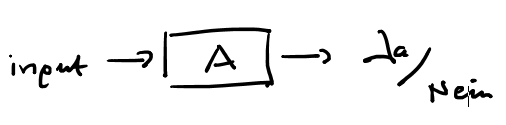
\includegraphics[width=6cm]{bild4.png}



Entscheidungsprobleme:

\begin{itemize}
\item Gibt es in einem Graphen eine Verbindung \\
von Knoten u nach Knoten v?
\item Hat dieses Sudoku eine Lösung?
\item Gegeben diese Schachstellung, kann Weiß sicher gewinnen?
\end{itemize}
\end{frame}

\begin{frame}[fragile]

P ist die Menge alle Entscheidungsprobleme, die sich  in polynomialer Zeit lösen lassen.   

NP umfasst alle Entscheidungsprobleme, die sich mit einem ``lucky algorithm'' in polynomialer Zeit lösen lassen.   

EXP umfasst alle Entscheidungsprobleme, die sich mit einem Algorithmus in exponentieller Zeit lösen lassen. 

R umfasst alle Entscheidungsprobleme, die sich in endlicher Zeit lösen lassen.  
\end{frame}
 

\begin{frame}[fragile]
``lucky algorithm'': ein nicht-deterministisches Modell eines Algorithmus, der im Lauf seiner Tätigkeit immer wieder ``guesses'' machen kann, die ihn zur richtigen Antwort führen.

\pause 
\begin{minipage}[c]{6cm}
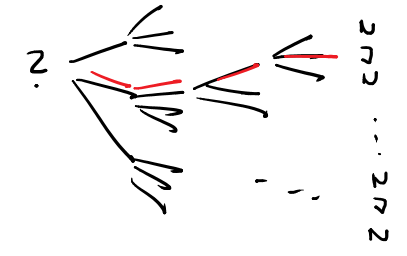
\includegraphics[width=6cm]{bild2.png}
\end{minipage} 
\begin{minipage}[c]{5cm}
Wenn es ein Ja gibt, dann findet der ``lucky algorithm'' garantiert einen Weg dorthin.
\end{minipage} 

 
Genauer: der Algorithmus darf unter polynomial vielen Optionen wählen, eine Wahl dauert O(1).
\end{frame}



\begin{frame}[fragile]
Das SAT-Problem: Gegeben ein boolescher Ausdruck. Gibt es eine Belegung seiner Variablen, so dass er sich 
zu True auswertet? \pause

Wir kennen keinen polynomialen Algorithmus, der das SAT-Problem löst. Aber es gibt einen ``lucky Algorithm'', der dieses Problem in polynomialer Zeit löst: Rate den Wert jeder Variablen, dann werte den booleschen Ausdruck aus.
\begin{lstlisting} 
rate $x_1$ = True oder False
rate $x_2$ = True oder False
...
if boolescher Ausdruck $==$ True: return JA
else: return NEIN
\end{lstlisting}  \pause

Wir stellen uns folgende Reihenfolge vor: Raten am Anfang, dann überprüfen, ob
das Geratene zu einem JA führt. Dadurch können wir uns das Ganze auch als Verifikations-Algorithmus vorstellen.
\end{frame}


\begin{frame}[fragile]

Ein Entscheidungsproblem ist in NP, wenn eine Lösung in polynomialer Zeit überprüft werden kann. \pause
\begin{itemize}
\item Eine Zahl faktorisieren ist schwer. Zu überprüfen, ob eine Faktorisierung stimmt, ist leicht. \pause
$\Rightarrow$  Faktorisierung  $\in$ NP

\item
 Ein Sudoku lösen ist schwer. Zu überprüfen, ob eine Lösung gültig ist, ist leicht.  \pause $\Rightarrow$  Sudoku  $\in$ NP
 
\item Zu einer gegebenen Stellung einen Gewinnzug für Weiß im Schach zu finden, ist schwer. Zu Überprüfen, ob die gefundene Lösung richtig ist, ist auch schwer. \pause $\Rightarrow$  Schach  $\notin$ NP
\end{itemize}
\end{frame}

\begin{frame}[fragile]
Stand heute: 

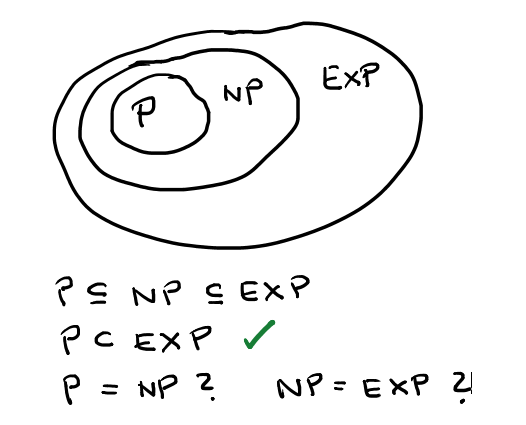
\includegraphics[width=8cm]{bild7.png}

\end{frame}



\begin{frame}[fragile]
Stephen Cook, 1971: SAT ist NP-vollständig, d.h;

1. SAT ist in NP \\
2. Jedes andere Problem in NP kann auf SAT reduziert werden (SAT ist NP-schwer).

Beispiel: das Clique-Problem ist in NP (Gibt es in einem Graphen G eine Clique der Größe k?). Jedes Clique-Problem kann transformiert werden in ein SAT-Problem mit äquivalenter Antwort.

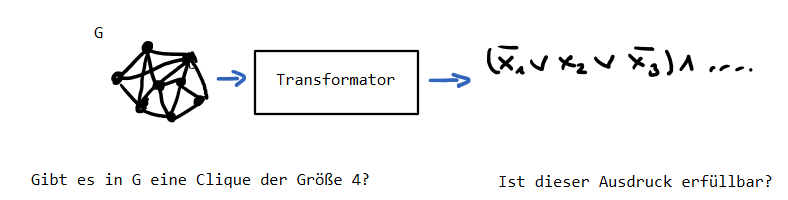
\includegraphics[width=12cm]{bild9.png}

\end{frame}

\begin{frame}[fragile]
Es gibt auch eine Reduktion von SAT auf Clique, also ist Clique auch NP vollständig. Inzwischen wurde für über
1000 Probleme gezeigt, dass sie NP vollständig sind. Wenn für eines dieser Probleme ein polynomialer
Algorithmus gefunden wird, sind auch alle anderen in polynomialer Zeit lösbar und es gilt $P = NP$.

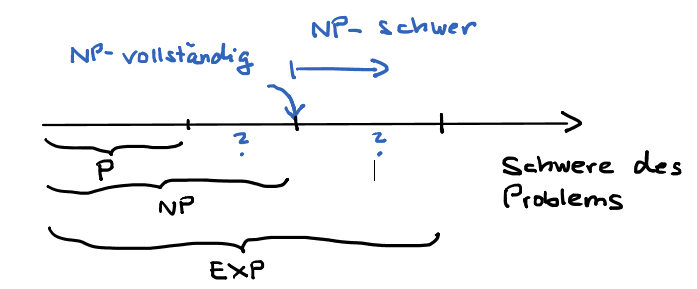
\includegraphics[width=9cm]{bild8.png}

\end{frame}

\begin{frame}[fragile]
Andere Formulierung: P = NP?  ist die Frage, ob man Suchprobleme auch ohne Suchen lösen kann. 

Kann man die Nadel im Heuhaufen finden, ohne im Heuhaufen zu suchen?  \pause Vielleicht mit einem großen Magnet?

Kann man herausfinden, ob eine Zahl eine Primzahl ist, ohne nach ihren Faktoren zu suchen?
\pause
Ja. \pause

Ist $p$ Primzahl und $a < p$, dann gilt: $a^{p-1}~\%~ p = 1$. (Kleiner Fermatscher Satz). Darauf basiert ein
Primzahltest, der in P ist (2002).




\end{frame}


 \end{document}
